\chapter{Beginning Algebra}

\section{Intro}

This course covers 9th grade math, i.e. the first year of high school mathematics.

\section{Polynomials}

There is no notes here.

\section{Multiplying Binomials}

FOIL = First terms, Outside terms, Inside terms, Last terms. Example: $(3x+3)(9x+4)$.

\section{Factoring Algebraic Expressions (Part I)}
%06 Sep 2025 trời chuẩn bị mưa

\begin{multicols}{2}
[
%optional header
  \textbf{Exercise}: Factor out the greatest common factor.
]

\begin{align*}
  \circled{1}\ &28x^{5}-8x^{3}+12x^{2}\\
  &=4x^{2}(7x^{3}-2x+3)
\end{align*}

\begin{align*}
  \circled{2}\ &21y^{4}-27y^{3}+15y\\
  &=3y(7y^{3}-9y^{2}+5)
\end{align*}

\begin{align*}
  \circled{3}\ &-50z^{6}+40z^{4}-15z^{3}\\
  &=-5z^{3}(10z^{3}-8z+3)
\end{align*}

\begin{align*}
  \circled{5}\ &-12y^{4}+33y^{3}-15y^{3}\\
  &=-3y^{3}(4y-11+5y^{2})
\end{align*}

\begin{align*}
  \circled{8}\ &24a^{5}b^{3}-18a^{2}-36a^{3}b^{2}\\
  &=6a^{2}(4a^{3}b^{3}-3-6ab^{2})
\end{align*}

\end{multicols}

In Problem \circled{3}, the leading term ($10z^{3}$) should be positive. Nên mình factor out the negative \& change the sign of the terms inside the parentheses.

\vspace{.6cm}

\begin{multicols}{2}
[
%optional header
  \textbf{Exercise}: Factor the quadratic expressions.
]

\begin{align*}
  \circled{15}\ &x^{2}+8x+15=(x+3)(x+5)\\
\end{align*}

  \[\circled{16}\ y^{2}+6y+5=(x+1)(x+5)\]

  \[\circled{18}\ x^{2}+8x+12=(x+2)(x+6)\]

  \[\circled{20}\ x^{2}+9x+18=(x+6)(x+3)\]

  \[\circled{26}\ z^{2}+3z-10=(z-2)(z+5)\]

  \[\circled{27}\ y^{2}-3y-28=(y-7)(y+4)\]

  \[\circled{28}\ x^{2}-15x+54=(x-6)(x-9)\]

  \[\circled{35}\ z^{2}-8z+15=(x-3)(x-5)\]

  \[\circled{29}\ z^{2}-7z-44=(z+4)(z-11)\]

  \[\circled{32}\ z^{2}+4z-21=(z+7)(z-3)\]

  \[\circled{37}\ z^{2}-12z+36=(z-6)(z-6)\]

  \[\circled{40}\ z^{2}+19z-20=(z+20)(z-1)\]

  \[\circled{42}\ x^{2}-x-12=(x+3)(x-4)\]

  \[\circled{46}\ z^{2}-13z+40=(z-8)(z-5)\]

  \[\circled{47}\ 2y^{2}+7y+3=(y+3)(2y+1)\]

  \[\circled{48}\ 3x^{2}+x-4=(3x+4)(x-1)\]

  \[\circled{49}\ 5z^{2}-6z+1=(5z-1)(z-1)\]

  \[\circled{50}\ 2y^{2}+7y+6=(2y+3)(y+2)\]

  \[\circled{51}\ 3x^{2}-10x-8=(3x+2)(x-4)\]

  \[\circled{52}\ 2y^{2}-7y-15=(2y+3)(y-5)\]

  \[\circled{55}\ 4y^{2}-17y+15=(4y-5)(y-3)\]

  \[\circled{57}\ 5z^{2}+18z-8=(5z-2)(z+4)\]

  \[\circled{31}\ 4b^{2}-35b+24=(4b-3)(b-8)\]
\end{multicols}

In Problem \circled{15}, ask yourself \q{\textbf{what two numbers multiply to 15 AND add up to 8?}} You can come up with ($1\cdot 15$) \& ($3\cdot 5$). But ($1+15=16 \neq 8$) nên chỉ còn lại 3 and 5.

Problem \circled{26} cũng làm theo cách tương tự. ($-2\cdot 5=-10$) AND ($-2+5=3$). If the last term of the trinomial is negative ($-10$), thì khi factor sẽ phải ra one positive \& one negative.

Problem \circled{28}, ta thấy last term is positive (54) but the second term is negtive ($-15x)$. Vậy khi factor phải ra 2 số âm.

Problem \circled{47}, you must ask two questions: \q{what two numbers multiply to 3?} \textbf{AND} \q{What two numbers multiply to 2?} First try $(y+1)(2y+3)=2y^{2}+5y+3$ is wrong. Now you switch the numbers: $(y+3)(2y+1)=2^{2}+7y+3$ is correct.

Problem \circled{48}, try these combinations: $(3x-2)(x+2)$; $(3x+2)(x-2)$; $(3x-1)(x+4)$; $(3x-4)(x+1)$; $(3x+4)(x-1)$. You have to try switching the numbers, try different multiplying combinations until you find the answer. If you get the right number for the middle term but the wrong sign (positive/negative) after FOIL-ing, you just change the signs.

\section{Factoring Algebraic Expressions (Part II)}
%07 Sep 2025 chủ nhật trời mưa

\begin{multicols}{2}
[
%optional header
  \textbf{Exercise}: Factoring the \hl{Difference of Two Squares}.
]

\begin{align*}
  \circled{1}\ x^{2}-16=(x-4)(x+4)
\end{align*}

  \[\circled{2}\ y^{2}-64=(y-8)(y+8)\]

  \[\circled{7}\ x^{2}-1=(x-1)(x+1)\]

  \[\circled{8}\ 4y^{2}-9=(2y-3)(2y+3)\]

  \[\circled{14}\ 36-x^{2}=(6-x)(6+x)\]

  \[\circled{20}\ -x^{2}+9=(3-x)(3+x)\]

\begin{align*}
  \circled{23}\ 81z^{4}-16&=(9z^{2}+4)(9z^{2}-4)\\
  &=(9z^{2}+4)(3z-2)(3z+2)
\end{align*}
\end{multicols}

Key Concept: $(x-3)(x+3)=x^{2}+3x-3x-9=x^{2}-9$

\vspace{.6cm}

\begin{multicols}{2}
[
%optional header
  \textbf{Exercise}: Factoring Quadratic Expressions with Two Variables and Factoring the Difference of Two Squares with Two Variables.
]

\begin{align*}
  \circled{24}\ x^{2}+8xy+15y^{2}=(x+3y)(x+5y)
\end{align*}

  \[\circled{25}\ x^{2}+2ab-63b^{2}=(a+9b)(a-7b)\]

  \[\circled{26}\ x^{2}-xy-30y^{2}=(x-6y)(x+5y)\]

  \[\circled{27}\ a^{2}+29ab-30b^{2}=(a+30b)(a-b)\]

  \[\circled{29}\ a^{2}-2ab+b^{2}=(a-b)(-b)\]

  \[\circled{30}\ x^{2}-4xy-45y^{2}=(x-9y)(x+5y)\]

  \[\circled{32}\ 2g^{2}-5gh-2h^{2}=(2g-h)(g-2h)\]

  \[\circled{33}\ 3x^{2}+10xz-8z^{2}=(3z-2z)(x+4z)\]

  \[\circled{34}\ 4x^{2}+19xz+12z^{2}=(4x+3z)(x+4z)\]

  \[\circled{37}\ 4a^{2}-20ab+9b^{2}=(2a-b)(2a-9b)\]

  \[\circled{39}\ 16a^{2}-25b^{2}=(4a-5b)(4a+5b)\]

  \[\circled{45}\ 9x^{2}-4y^{2}=(3x-2y)(3x+2y)\]
\end{multicols}

In problem \circled{1}, cũng lại ask yourself \q{what two numbers multiply to 15 AND add up to 8?} Nhưng vì có 2 variables nên phải viết thêm biến $y$ vô nữa.

\section{Factoring Algebraic Expressions (Part III)}
% 07 Sep 2025 chủ nhật trời mưa âm u lắm, rằm vu lang tháng 7

\begin{multicols}{2}
[
%optional header
  \textbf{Exercise}: Factoring Trinomials of the Form $ax^{4}+bx^{2}+c$.
]

\begin{align*}
  \circled{1}\ x^{4}+13x^{2}+40=(x^{2}+5)(x^{2}+8)
\end{align*}

\begin{align*}
  \circled{2}\ y^{4}-4y^{2}-45&=(y^{2}-9)(y^{2}+5)\\
  &=(y-3)(y+3)(y^{2}+5)
\end{align*}

\begin{align*}
  \circled{4}\ &a^{4}-13a^{2}+36\\
  &=(a^{2}-9)(a^{2}-4)\\
  &=(a-3)(a+3)(a-2)(a+2)
\end{align*}

\begin{align*}
  \circled{7}\ z^{4}-5z^{2}+4&=(z^{2}-1)(z^{2}-4)\\
  &=(z-1)(z+1)(z-2)(z+2)
\end{align*}

\begin{align*}
  \circled{17}\ 2x^{4}+11x^{2}+5=(2x^{2}+1)(x^{2}+5)\\
\end{align*}

  \[\circled{18}\ 3y^{4}+10y^{2}-25=(3y^{2}-5)(y^{2}+5)\]

  \[\circled{20}\ 8x^{4}+2x^{2}-3=(4x^{2}+3)(2x^{2}-1)\]

\begin{align*}
  \circled{21}\ &9y^{4}-25y^{2}+16\\
  &=(9y^{2}-16)(y^{2}-1)\\
  &=(3y-4)(3y+4)(y-1)(y+1)
\end{align*}
\end{multicols}

\vspace{.6cm}

\begin{multicols}{2}
[
%optional header
  \textbf{Exercise}: Factoring by Grouping.
]

\begin{align*}
  \circled{22}\ &x^{3}+4x^{2}+4x+16\\
  &x^{2}(x+4)+4(x+4)\\
  &(x+4)(x^{2}+4)
\end{align*}

\begin{align*}
  \circled{23}\ &6y^{3}-10y^{2}+9y-15\\
  &2y^{2}(3y-5)+3(3y-5)\\
  &(3y-5)(2y^{2}+3)
\end{align*}

\begin{align*}
  \circled{24}\ &z^{5}-z^{4}-81z+81\\
  &z^{4}(z-1)-81(z-1)\\
  &(z-1)(z^{4}-81)\\
  &(z-1)(z^{2}+9)(z^{2}-9)\\
  &(z-1)(z^{2}+9)(z-3)(z+3)
\end{align*}

\begin{align*}
  \circled{26}\ &12y^{4}-6y^{3}+2y-1\\
  &6y^{3}(2y-1)+1(2y-1)\\
  &(2y-1)(6y^{3}+1)\\
\end{align*}

\begin{align*}
  \circled{29}\ &5z^{3}-35z^{2}-z+7\\
  &5z^{2}(z-7)-1(z-7)\\
  &(z-7)(5z^{2}-1)\\
\end{align*}

\begin{align*}
  \circled{31}\ &2x^{6}-18z^{5}-z+9\\
  &2z^{5}(z-9)-1(z-9)\\
  &(z-9)(2z^{5}-1)\\
\end{align*}
\end{multicols}

\section{Factoring Algebraic Expressions (Part IV)}
%08 Sep 2025 trời mưa

\begin{multicols}{2}
[
%optional header
  \textbf{Exercise}: Combined Types of Factoring.
]

\begin{align*}
  \circled{1}\ &6x^{4}+18x^{3}+12x^{2}\\
  &6x^{2}(x^{2}+3x+2)\\
  &6x^{2}(x+2)(x+1)
\end{align*}

\begin{align*}
  \circled{3}\ &-12x^{8}-4x^{7}+8x^{6}\\
  &-4x^{6}(3x^{2}+x-2)\\
  &-4x^{6}(3x+2)(x-1)
\end{align*}

\begin{align*}
  \circled{7}\ &-6z^{3}+38z^{2}-60z\\
  &-2z(3z^{2}-19z+30)\\
  &-2z(3z-10)(z-3)
\end{align*}

\begin{align*}
  \circled{11}\ &4y^{3}+4y^{2}-120y\\
  &4y(y^{2}+y-30)\\
  &4y(y+6)(y-5)
\end{align*}

\begin{align*}
  \circled{13}\ &-18x^{6}+18x^{5}+8x^{4}\\
  &-2x^{4}(9x^{2}-9x-4)\\
  &-2x^{4}(3x+1)(3x-4)
\end{align*}

\begin{align*}
  \circled{18}\ &4x^{6}+16x^{5}+6x^{3}+24x^{2}\\
  &2x^{2}(2x^{4}+8x^{3}+3x+12)\\
  &2x^{2}[2x^{3}(x+4)+3(x+4)]\\
  &2x^{2}(x+4)(2x^{3}+3)\
\end{align*}

\begin{align*}
  \circled{19}\ &-y^{8}-5y^{6}+3y^{5}+15y^{3}\\
  &-y^{3}(y^{5}+5y^{3}-3y^{2}-15)\\
  &-y^{3}[y^{3}(y^{2}+5)-3(y^{2}+5)]\\
  &-y^{3}(y^{2}+5)(y^{3}-3)\
\end{align*}

\begin{align*}
  \circled{22}\ &-2x^{5}-3x^{3}+44x\\
  &-x(2x^{4}+3x^{2}-44)\\
  &-x(2x^{2}+11)(x^{2}-4)\\
  &-x(2x^{2}+11)(x-2)(x+2)
\end{align*}

\begin{align*}
  \circled{26}\ &2a^{4}b^{5}+16a^{3}b^{6}+24a^{2}b^{7}\\
  &2a^{2}b^{5}(a^{2}+8ab+12b^{2})\\
  &2a^{2}b^{5}(a+2b)(a+6b)\\
\end{align*}

\begin{align*}
  \circled{27}\ &4x^{10}y^{6}-100x^{8}y^{8}\\
  &4x^{8}y^{6}(x^{2}-25y^{2})\\
  &4x^{8}y^{6}(x-5y)(x+5y)\\
\end{align*}

\begin{align*}
  \circled{28}\ &-6c^{7}d^{2}-15c^{6}d^{3}+9c^{5}d^{4}\\
  &-3c^{5}d^{2}(2c^{2}+5cd-3d^{2})\\
  &-3c^{5}d^{2}(2c-d)(c+3d)\\
\end{align*}
\end{multicols}

In problem \circled{3}, you should always factor out the negative sign on the first term. That makes it easier to solve the problem.

\section{Solving Quadratic Equations by Factoring}
%10 Sep 2025 trời nắng đẹp

\begin{multicols}{2}
[
%optional header
  \textbf{Exercise}: Solve the following quadratic equations.
]

\begin{align*}
  \circled{1}\ x^{2}+6x+8&=0\\
  (x+4)(x+2)&=0\\
  x+4=0 \text{ or }&x+2=0\\
  x=-4 \text{ or }&x=-2
\end{align*}

\begin{align*}
  \circled{21}\ 6y^{2}-13y-28&=0\\
  (2y-7)(3y+4)&=0\\
  2y-7=0 \text{ or }&3y+4=0\\
  y=\frac{7}{2} \text{ or }&y=-\frac{4}{3}
\end{align*}
\end{multicols}

\section{Solving Equations with Squares}
%11 Sep 2025

\begin{multicols}{2}
[
%optional header
  \textbf{Exercise}: Solve.
]

\begin{align*}
  \circled{1}\ x^{2}&=36\\
  \sqrt{x^{2}}&=\pm\sqrt{36}\\
  x&=\pm 6
\end{align*}

\begin{align*}
  \circled{5}\ 7&=z^{2}+6\\
  1&=z^{2}\\
  \pm\sqrt{1}&=\sqrt{z^{2}}\\
  z&=\pm 1
\end{align*}

\begin{align*}
  \circled{6}\ 9&=7+z^{2}\\
  2&=z^{2}\\
  \pm\sqrt{2}&=\sqrt{z^{2}}\\
  z&=\pm \sqrt{2}
\end{align*}

\begin{align*}
  \circled{7}\ 4&=3y^{2}\\
  \frac{4}{3}&=y^{2}\\
  \pm\sqrt{\frac{4}{3}}&=\sqrt{y^{2}}\\
  y&=\pm \frac{2\sqrt{3}}{3}
\end{align*}

\begin{align*}
  \circled{10}\ -3+8y^{2}&=4\\
  y^{2}&=\frac{7}{8}\\
  \sqrt{y^{2}}&=\pm\sqrt{\frac{7}{8}}\\
  y&=\pm\frac{\sqrt{14}}{4}
\end{align*}

\begin{align*}
  \circled{11}\ (a+3)^{2}+6&=8\\
  (a+3)^{2}&=2\\
  \sqrt{(a+3)^{2}}&=\pm\sqrt{2}\\
  a+3&=\pm\sqrt{2}\\
  a&=-3\pm\sqrt{2}
\end{align*}

\begin{align*}
  \circled{15}\ 7&=\frac{(x+3)^{2}}{9}+2\\
  45&=(x+3)^{2}\\
  \pm\sqrt{45}&=\sqrt{(x+3)^{2}}\\
  \pm 3\sqrt{5}&=x+3\\
  x&=\pm 3\sqrt{5}-3
\end{align*}

\begin{align*}
  \circled{20}\ \frac{(z-5)^{2}}{2}+12&=21\\
  (z-5)^{2}&=18\\
  \sqrt{(z-5)^{2}}&=\pm\sqrt{18}\\
  z-5&=\pm 3\sqrt{2}\\
  z&=5\pm 3\sqrt{2}
\end{align*}

\begin{align*}
  \circled{22}\ 4(x-3)^{2}-6&=10\\
  (x-3)^{2}&=4\\
  \sqrt{(x-3)^{2}}&=\pm\sqrt{4}\\
  x-3&=\pm 2\\
  x&=\pm 2+3\\
  x=5 &\text{ or }x=1
\end{align*}

\begin{align*}
  \circled{33}\ 24&=27(x+2)^{2}+4\\
  \frac{20}{27}&=(x+2)^{2}\\
  \pm\sqrt{\frac{20}{27}}&=\sqrt{(x+2)^{2}}\\
  \pm \frac{2\sqrt{5}}{3\sqrt{3}}&=x+2\\
  \pm \frac{2\sqrt{15}}{9}-2&=x
\end{align*}

\begin{align*}
  \circled{35}\ 16&=\frac{(3y+2)^{2}}{4}+8\\
  32&=(3y+2)^{2}\\
  \pm\sqrt{32}&=\sqrt{(3y+2)^{2}}\\
  \pm 4\sqrt{2}&=3y+2\\
  \frac{\pm 4\sqrt{2}-2}{3}&=y\\
\end{align*}

\begin{align*}
  \circled{37}\ -4&=5(\frac{z}{2}-3)^{2}-7\\
  \frac{3}{5}&=(\frac{z}{2}-3)^{2}\\
  \pm \sqrt{\frac{3}{5}}&=\sqrt{(\frac{z}{2}-3)^{2}}\\
  \pm \frac{\sqrt{15}}{5}&=\frac{z}{2}-3\\
  \pm \frac{\sqrt{15}}{5}+3&=\frac{z}{2}\\
  \pm \frac{2\sqrt{15}}{5}+6&=z
\end{align*}

\begin{align*}
  \circled{38}\ \frac{(1-\frac{x}{3})^{2}}{3}-9&=1\\
  (1-\frac{x}{3})^{2}&=30\\
  \sqrt{(1-\frac{x}{3})^{2}}&=\pm\sqrt{30}\\
  1-\frac{x}{3}&=\pm\sqrt{30}\\
  \frac{x}{-3}&=\pm\sqrt{30}-1\\
  x&=(\pm\sqrt{30}-1)(-3)\\
  x&=\pm 3\sqrt{30}+3
\end{align*}

\begin{align*}
  \circled{22}\ \text{(homework):}\ 17&=1+(\frac{x}{4}-7)^{2}\\
  16&=(\frac{x}{4}-7)^{2}\\
  \pm 4&=\frac{x}{4}-7\\
  \pm 4+7&=\frac{x}{4}\\
  x&=\pm 16+28\\
  x=44 &\text{ or }x=12
\end{align*}
\end{multicols}

In problem \circled{38}, $(-3)\times(\pm\sqrt{30})=\pm 3\sqrt{30}$ không có đổi dấu gì hết, the result is the same. Just remember when negative multiply a plus-and-minus thì the negative sign goes away.

\section{Solving Equations with Fractions}
%12 Sep 2025 a normal day, deploy docusaurous with a sub-domain notes.anhaopham.com

\begin{multicols}{2}
[
%optional header
  \textbf{Exercise}: Solve.
]

\begin{align*}
  \circled{1}\ 2x+\frac{1}{6}&=-\frac{1}{2}+\frac{15x}{18}\\
  \frac{36x}{18}+\frac{3}{18}&=-\frac{9}{18}+\frac{15x}{18}\\
  \frac{36x+3}{18}&=\frac{-9+15x}{18}\ \text{ (*)}\\
  36x+3&=-9+15x\\
  x&=-\frac{12}{21}=-\frac{4}{7}
\end{align*}

\begin{align*}
  \circled{4}\ \frac{3}{4}-\frac{z}{2}&=3z-2\\
  \frac{3}{4}-\frac{2z}{4}&=\frac{12z}{4}-\frac{8}{4}\\
  \frac{3-2z}{4}&=\frac{12z-8}{4}\\
  3-2z&=12z-8\\
  z&=\frac{11}{14}
\end{align*}

\begin{align*}
  \circled{7}\ \frac{2}{5y}+\frac{1}{10}&=3-\frac{4}{y}\\
  \frac{4+y}{10y}&=\frac{30y-40}{10y}\\
  4+y&=30y-40\\
  y&=\frac{44}{29}
\end{align*}

\begin{align*}
  \circled{11}\ z=4&=\frac{45}{z}\\
  \frac{z^{2}-4z}{z}&=\frac{45}{z}\\
  z^{2}-4z-45&=0\\
  (z-9)(z+5)&=0\\
  z=9 \text{ or }&z=-5
\end{align*}

\begin{align*}
  \circled{13}\ -\frac{15}{2x}&=x+\frac{11}{2}\\
  \frac{-15}{2x}&=\frac{2x^{2}+11x}{2x}\\
  0&=2x^{2}+11x+15&\\
  0&=(2x+5)(x+3)\\
  x=&-\frac{5}{2} \text{ or }x=-3
\end{align*}

\begin{align*}
  \circled{14}\ \frac{5y}{2}+\frac{10}{y}&=-14.5\\
  \frac{5y^{2}}{2y}+\frac{20}{2y}&=\frac{-29y}{2y}\\
  5y^{2}+29y+20&=0\\
  (5y+4)(y+5)&=0\\
  y=-\frac{4}{5} &\text{ or }y=-5
\end{align*}

\begin{align*}
  \circled{19}\ \frac{2}{x-1}+\frac{x-6}{2x^{2}+5x-7}&=\frac{3}{2x+7}\\
  \frac{2}{x-1}+\frac{x-6}{(2x+7)(x-1)}&=\frac{3}{2x+7}\\
  \frac{2(2x+7)+(x-6)}{(2x+7)(x-1)}&=\frac{3(x-1)}{(2x+7)(x-1)}\\
  \frac{5x+8}{(2x+7)(x-1)}&=\frac{3x-3}{(2x+7)(x-1)}\\
  5x+8&=3x-3\\
  x&=-\frac{11}{2}
\end{align*}

\begin{align*}
  \circled{23}\ \frac{7}{2z^{2}-10z}+\frac{-1}{z}&=\frac{1}{z-5}\\
  \frac{7}{2z(z-5)}+\frac{(-1)\cdot 2(z-5)}{2z(z-5)}&=\frac{1(2z)}{2z(z-5)}\\
  \frac{7-2z+10}{2z(z-5)}&=\frac{2z}{2z(z-5)}\\
  7-2z+10&=2z\\
  z&=\frac{17}{4}
\end{align*}

\begin{align*}
  \circled{25}\ \frac{1}{x-1}+\frac{x}{x-8}&=\frac{-7}{x^{2}-9x+8}\\
  \frac{1}{x-1}+\frac{x}{x-8}&=\frac{-7}{(x-8)(x-1)}\\
  \frac{1(x-8)+x(x-1)}{(x-8)(x-1)}&=\frac{-7}{(x-8)(x-1)}\\
  x^{2}&=1\\
  \sqrt{x^{2}}&=\pm\sqrt{1}\\
  x&=\pm 1\\
  x\neq 1 &\text{ or } x=-1
\end{align*}

\begin{align*}
  \circled{26}\ \frac{-4}{x^{2}+14x+45}&=\frac{1}{x+9}+\frac{x}{x+5}\\
  \frac{-4}{(x+9)(x+5)}&=\frac{1}{x+9}+\frac{x}{x+5}\\
  \frac{-4}{(x+9)(x+5)}&=\frac{1(x+5)+x(x+9)}{(x+9)(x+5)}\\
  x^{2}+10x+9&=0\\
  (x+9)(x+1)&=0\\
  x\neq-9 &\text{ or } x=-1
\end{align*}

\begin{align*}
  \circled{29}\ \frac{x+3}{16x^{2}-9}+\frac{2}{4x+3}&=\frac{1}{4x-3}\\
  \frac{x+3}{(4x-3)(4x+3)}+\frac{2}{4x+3}&=\frac{1}{4x-3}\\
  \frac{(x+3)+2(4x-3)}{(4x-3)(4x+3)}&=\frac{1(4x+3)}{(4x-3)(4x+3)}\\
  5x-6&=0\\
  x&=\frac{6}{5}
\end{align*}

\begin{align*}
  \circled{31}\ \frac{9}{x^{2}-5x+4}&=\frac{1}{x-1}+\frac{3}{x-4}\\
  \frac{9}{(x-4)(x-1)}&=\frac{1}{x-1}+\frac{3}{x-4}\\
  \frac{9}{(x-4)(x-1)}&=\frac{1(x-4)+3(x-1)}{(x-4)(x-1)}\\
  9&=4x-7\\
  4&\neq x\ \text{ [No Solution]}
\end{align*}

\begin{align*}
  \circled{23}\ \text{(homework)}&\\
  \frac{4}{y-1}-\frac{4}{y+1}-\frac{7}{y^{2}-1}&=\frac{y^{2}}{y^{2}-1}\\
  \frac{4(y+1)-4(y-1)-7}{(y-1)(y+1)}&=\frac{y^{2}}{(y-1)(y+1)}\\
  1&=y^{2}\\
  \pm 1&=y\ \text{ [No Solution]}\\
\end{align*}
\end{multicols}

In Problem \circled{1}, step (*), since the denominators are the same (18), the numerators must also be equal. So we can get rid of the denominator.

\vspace{.4cm}

An \hl{extraneous solution} is a value obtained during the process of solving an equation that does not actually satisfy the original equation when you plug it back in.

An extraneous solution for an equation with fractions is any solution that would make the denominators zero. So in problem \circled{7}, the extraneous solution, if exists, would be $y=0$. But the solution we found is $\frac{44}{29}$. Therefore it is correct.

In problem \circled{19}, the two extraneous solutions, if exists, would be $2x+7=0\leftrightarrow x=-\frac{7}{2}$ \& $x-1=0 \leftrightarrow x=1$.

In problem \circled{25}, $x=1$ is an extraneous solution, so we must exclude it in the final answer.

In problem \circled{31}, the only solution is extraneous, so the equation has no solution.

\section{Solving More Equations by Factoring}
%15 Sep 2025, trời rất nắng, buổi chiều hoàng hôn màu vàng, bà nội xay chanh & xả uống

\begin{multicols}{2}
[
%optional header
  \textbf{Exercise}: Solve.
]

\begin{align*}
  \circled{1}\ 3x^{3}+21x^{2}+30x&=0\\
  3x(x^{2}+7x+10)&=0\\
  3x(x+5)(x+2)&=0\\
  x=0 \text{ or }x=-2 &\text{ or }x=-5
\end{align*}

\begin{align*}
  \circled{6}\ z^{8}-8z^{7}+16z^{6}&=0\\
  z^{6}(z^{2}-8z+16)&=0\\
  z^{6}(z-4)(z-4)&=0\\
  z=0 \text{ or }z=4
\end{align*}

\begin{align*}
  \circled{9}\ -12x^{8}-4x^{7}+8x^{6}&=0\\
  -4x^{6}(3x^{2}+x-2)&=0\\
  -4x^{6}(3x-2)(x+1)&=0\\
  x=0 \text{ or }x=\frac{2}{3} \text{ or }&x=-1
\end{align*}

\begin{align*}
  \circled{11}\ -6z^{3}+38z^{2}-60z&=0\\
  -2z(3z^{2}-19z+30)&=0\\
  -2x(3z-10)(z-3)&=0\\
  z=0 \text{ or }z=\frac{10}{3} \text{ or }&z=3
\end{align*}

\begin{align*}
  \circled{18}\ x^{3}+10x^{2}-4x-40&=0\\
  x^{2}(x+10)-4(x+10)&=0\\
  (x+10)(x^{2}-4)&=0\\
  (x+10)(x-2)(x+2)&=0\\
  x=-10 \text{ or }x=2 \text{ or }&x=-2
\end{align*}

\begin{align*}
  \circled{22}\ x^{3}+4x^{2}+4x+16&=0\\
  x^{2}(x+4)+4(x+4)&=0\\
  (x+4)(x^{2}+4)&=0\\
  x+4=0 \text{ | } x^{2}+4&=0\\
  x=-4 \text{ | } x^{2}\neq&-4\\
\end{align*}

\begin{align*}
  \circled{24}\ 5z^{3}-35z^{2}-z+7&=0\\
  5z^{2}(z-7)-1(z-7)&=0\\
  (z-7)(5z^{2}-1)&=0\\
  z-7=0 \text{ | } 5z^{2}-1&=0\\
  z=7 \text{ | } z=\pm \frac{\sqrt{5}}{5}&\\
\end{align*}

\begin{align*}
  \circled{26}\ -2x^{5}-3x^{3}+44x&=0\\
  -x(2x^{4}+3x^{2}-44)&=0\\
  -x(2x^{2}+11)(x^{2}-4)&=0\\
  -x(2x^{2}+11)(x-2)(x+2)&=0\\
  x=0 \text{ | } 2x^{2}+11=0\ \text{ | }x&=\pm 2\\
  x=0 \text{ | } x^{2}\neq -\frac{11}{2}\ \text{ | }x&=\pm 2\\
\end{align*}

\begin{align*}
  \circled{28}\ 5z^{7}-5z^{3}&=0\\
  5z^{3}(z^{4}-1)&=0\\
  5z^{3}(z^{2}-1)(z^{2}+1)&=0\\
  5z^{3}(z-1)(z+1)(z^{2}+1)&=0\\
  z=0 \text{ | } z=\pm 1\ \text{ | }z^{2}&\neq -1\\
\end{align*}

\begin{align*}
  \circled{35}\ -9y+15&=6y^{3}-10y^{2}\\
  0&=6y^{3}-10y^{2}+9y-15\\
  0&=2y^{2}(3y-5)+3(3y-5)\\
  0&=(3y-5)(2y^{2}+3)\\
  y&=\frac{5}{3} \text{ | } y\neq -\frac{3}{2}\\
\end{align*}
\end{multicols}

\section{Solving Equations with Square Roots}
%19-sep-2025 hôm qua mới lên quận 1 coding interview với mẹ Yến

\centerline{\colorbox{yellow}{\underline{\textbf{\large Equations with One Square Root}}}}

\vspace{.5cm}

\begin{multicols}{2}
[
%optional header
  \textbf{Exercise}: Solve.
]

\begin{align*}
  \circled{1}\ \sqrt{x}-4&=-2\\
  \sqrt{x}&=2\\
  (\sqrt{x})^{2}&=2^{2}\\
  x&=4
\end{align*}

\begin{align*}
  \circled{7}\ 7\sqrt{x}-1&=13\\
  \sqrt{x}&=2\\
  (\sqrt{x})^{2}&=2^{2}\\
  x&=4
\end{align*}

\begin{align*}
  \circled{8}\ -10&=\sqrt{x-3}-4\\
  -6&=\sqrt{x-3}\ \text{ (No solution)}\\
\end{align*}

\begin{align*}
  \circled{16}\ 4&=\sqrt{3-2x}+2\\
  2&=\sqrt{3-2x}\\
  2^{2}&=(\sqrt{3-2x})^{2}\\
  4&=3-2x\\
  -\frac{1}{2}&=x
\end{align*}

\begin{align*}
  \circled{17}\ 8&=7+\frac{\sqrt{2z-4}}{-3}\\
  -3&=\sqrt{2z-4}\ \text{ (No solution)}\\
\end{align*}

\begin{align*}
  \circled{21}\ 0&=\sqrt{2y^{2}+3y+1}\\
  0^{2}&=(\sqrt{2y^{2}+3y+1})^{2}\\
  0&=2y^{2}+3y+1\\
  0&=(2y+1)(y+1)\\
  y&=-\frac{1}{2} \text{ or } y=-1
\end{align*}

\begin{align*}
  \circled{23}\ x+4&=\sqrt{3x+10}\\
  (x+4)^{2}&=(\sqrt{3x+10})^{2}\\
  x^{2}+8x+16&=3x+10\\
  x^{2}+5x+6&=0\\
  (x+3)(x+2)&=0\\
  x=-3 \text{ or } x&=-2
\end{align*}

\begin{align*}
  \circled{28}\ 5&=\sqrt{7-z}-z\\
  z+5&=\sqrt{7-z}\\
  (z+5)^{2}&=(\sqrt{7-z})^{2}\\
  z^{2}+11z+18&=0\\
  (z+9)(z+2)&=0\\
  z\neq-9 \text{ or } z&=-2
\end{align*}
\end{multicols}

In problem \circled{8}, since the radical symbol only produce positive result, there is no solution. Cái notation này nó được quy ước như vậy phải chấp nhận (luật chơi nó vậy don't ask question!).

In problem \circled{23}, nhớ phải plug your answers (-3 and -2) back in the original equation ($x+4=\sqrt{3x+10}$) to check for any extraneous solution. Vì phương trình này phức tạo nên phải làm như vậy.

In problem \circled{28}, when you plug (-9) back into $5=\sqrt{7-z}-z$, you get $5=13$, so (-9) is an extraneous solution.

\vspace{.4cm}

Remember $-6^{2}\neq(-6)^{2}$ because $-6^{2}=-36$ while $(-6)^{2}=36$.

\vspace{.8cm}

\centerline{\colorbox{yellow}{\underline{\textbf{\large Equations with Two Square Roots}}}}

\vspace{.5cm}

\begin{multicols}{2}
[
%optional header
  \textbf{Exercise}: Solve.
]

\begin{align*}
  \circled{29}\ \sqrt{y}&=\sqrt{2y-5}\\
  (\sqrt{y})^{2}&=(\sqrt{2y-5})^{2}\\
  y&=2y-5\\
  y&=5\\
\end{align*}
\end{multicols}

\section{Solving Systems of Equations}
% 07 Aug 2025

% \vspace{1 cm}
%
% \centerline{\textbf{\large System of Equations with No Solution or Infinite Solutions}}
%
% \vspace{0.2 cm}

System of Equations can have: một cặp nghiệm (x,y), no Solution or Infinite Solutions.

\vspace{.4cm}

There are three methods for solving systems of Equations:

\begin{enumerate}
  \item Substitution: lấy 1 phương trình dễ tìm x theo y, sau đó thay x vừa tìm vào phương trình còn lại tìm y.
  \item Elimination: cộng hoặc trừ 2 phương trình lại với nhau để khử đi một biến
  \item Graphing
\end{enumerate}

Only Substitution \& Elimination được dùng in the real world. Graphing is really not practical, takes too long, not reliable.

% \begin{equation}
%   \begin{cases}
%     x+4y = 5\\
%     x-4y=-3
%   \end{cases} \iff
%   \begin{cases}
%     x+4y = 5\\
%     x-4y=-3
%   \end{cases} \iff
% \end{equation}

Example of Solving by Elimination (Addition or Subtraction)

% `\right.` is a "phantom" right delimiter
\[
  \begin{aligned}
    &\left\{\begin{aligned} 
      x + 4y &= 5 \\ 
      x - 4y &= -3
    \end{aligned}\right. \iff 
    \left\{\begin{aligned}
      &x +4y = 5\\ 
      &2x = 2
    \end{aligned}\right.
    \\
    \iff &\left\{\begin{aligned} 
      x &= 1 \\ 
      y &= 1
    \end{aligned}\right.
  \end{aligned}
\]

\newpage

Phương pháp elimination, đôi khi phải multiply both equation.

\begin{figure}[htb!]
  \centering
  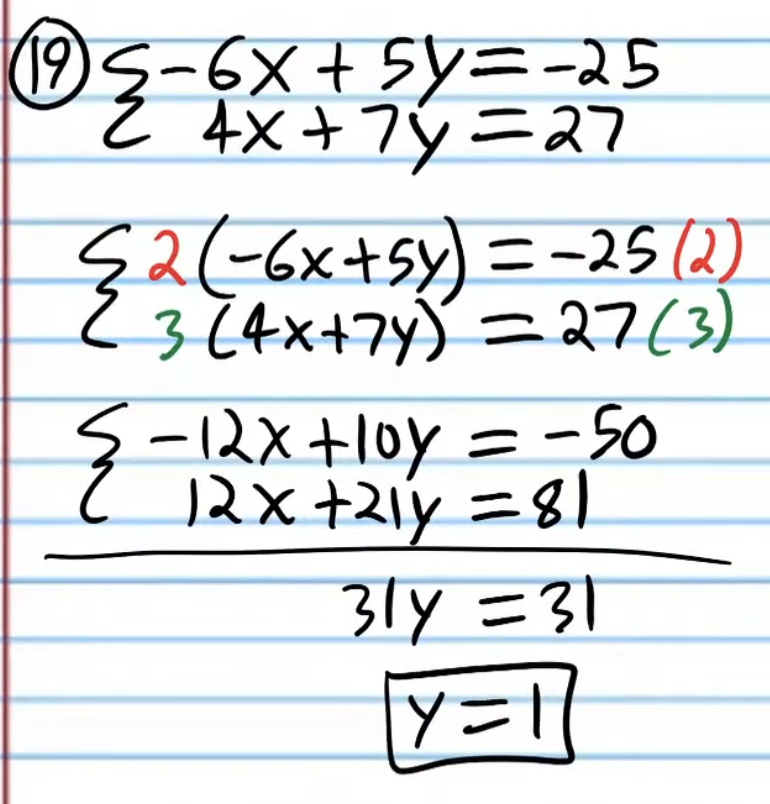
\includegraphics[width=0.4\textwidth]{int0201.png}
  \caption{bài tập}
\end{figure}

Graphical representations of System of Equations.

\begin{figure}[htb!]
  \centering
  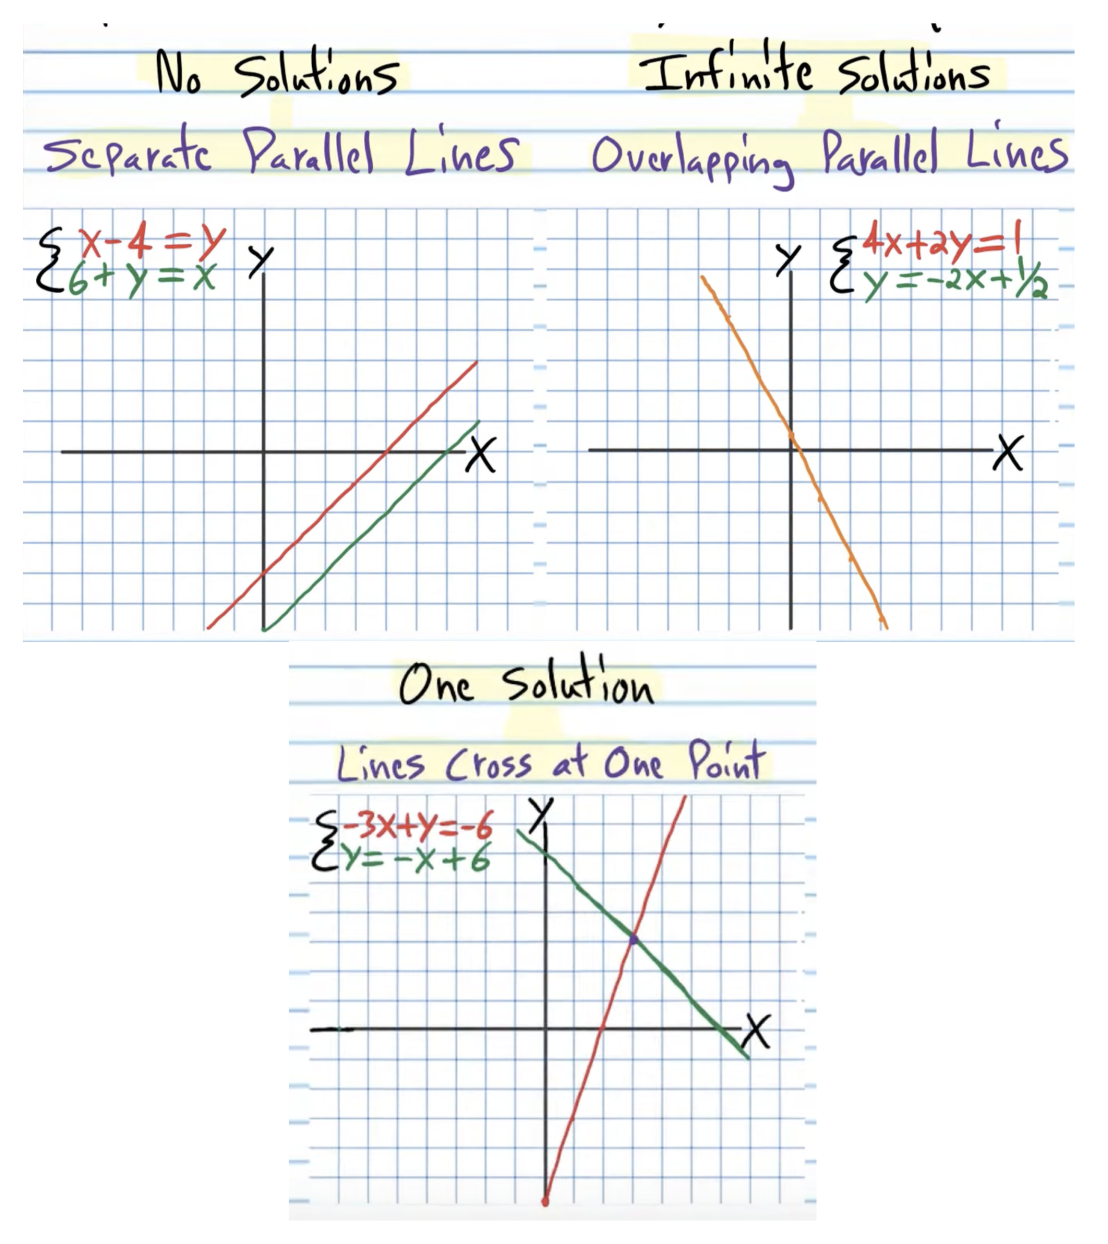
\includegraphics[width=0.6\textwidth]{int0202.png}
  \caption{Graphical representations of sys of Eq}
\end{figure}

\newpage

\section{The Three Forms of Linear Equations and Finding Slope}

% \vspace{1 cm}

% \centerline{\textbf{\large The Slope of a Line}}

% \vspace{0.2 cm}

If \(A(x_{1},y_{1})\text{ and } B(x_{2},y_{2})\) are two points on a line, \textbf{the slope of the line} is defined by the equation below.

\begin{equation}
  m = \frac{y_{2}-y_{1}}{x_{2}-x_{1}}
  \label{eq:3.1}
\end{equation}

\hl{Slope} (hệ số góc) measures the steepness of a line. If the slope of a line is positive, the line travels up moving from left to right. If the slope of a line is negative, the line travels down moving left to right. If the slope of a line is zero, the line is horizontal. If the slope of a line is undefined, the line is vertical.

\textbf{Slope} (hệ số góc) cho biết rate of change. Two parallel lines have \textit{the same} slope.

% \newpage

\begin{figure}[htb!]
  \centering
  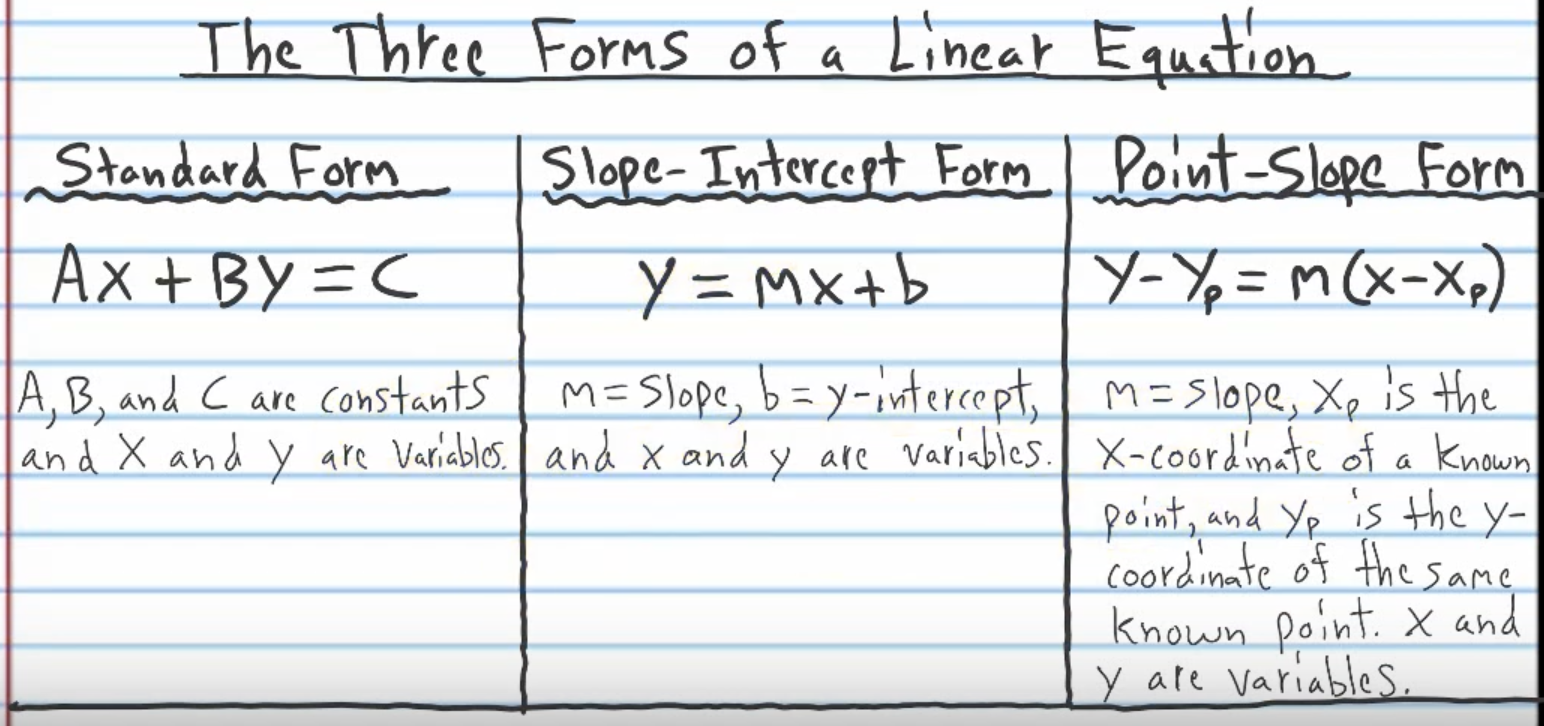
\includegraphics[width=1\textwidth]{beg2601.png}
  \caption{The Three Forms of a Linear Equation}
\end{figure}

% \par\rule{\textwidth}{0.5pt}

% \vspace{1cm}

\textbf{Excercise}: Identify the form of each linear equation below by writing \q{S} for Standard, \q{SI} for slope-intercept, or \q{PS} for point-slope.

$2x+4y=3$: \textbf{S} because the variables x and y are on the same side of the equation.

$4=-8x+7x$: still Standard form, even though the equation is flipped.

$y-4=-3(x-5)$: \textbf{PS}, it is the only form that has parenthesses.

$y=2x+4$: \textbf{SI}, because the y is isolated on one side of the equation.

% \par\rule{\textwidth}{0.5pt}

\vspace{.6cm}

The standard form is not really useful for graphing. Nó không cho biết point, slope or y-intercept. Khi nhìn thấy standard form (x and y on the same side), convert into slope-Intercept form (where y is isolated). Slope-Intercept is the most useful form of the linear equation. Nó cho mình biết slope \& y-intercept.

You also need to be able to convert from Point-slope form to Slope-intercept form. Cách làm cũng là isolate y về một bên.

% Below is not from the course

\vspace{2 cm}

\textbf{Q:} Graph this line \(3x-4y=-6\)

Find the \textbf{x-intercept} by making y = 0. Then find the \textbf{y-intercept} by making x = 0.

\vspace{5mm}

\textbf{Q:} Graph this inequality \(y < -\frac{1}{3}x+2\)

Tìm tọa độ 2 điểm; vẽ đường thẳng.

\begin{itemize}
  \item Nếu \(\le\) thì vẽ straight line and shade under the line.
  \item Nếu > thì vẽ dashed line and shade above the line.
\end{itemize}

\textbf{Q: }Graphing Systems of Inequalities

\vspace{5mm}

Tính \textbf{Distance between 2 points} bằng Eq \ref{eq:3.2} below:

\begin{equation}
  d = \sqrt{(x_{1}-x_{2})^{2} + (y_{1}-y_{2})^{2}}
  \label{eq:3.2}
\end{equation}

\section{Graphing Linear Equations}

\hl{Method 01}: Finding two random points.

\hl{Method 02}: Finding x and y intercepts. Làm giống method 01 nhưng must chose $x=0$ and $y=0$. Useful when dealing with standard form.

% \vspace{4cm}

\hl{Method 03}: Convert to Slope-Intercept form and use slope and y-intercept.

The slope is $\frac{\text{rise}}{\text{run}}$. In the figure below, first we find that the y-intercept is $(0,-1)$. Then we rise up two and run to the right 3 to get to the second point of $(3,1)$.

\begin{figure}[htb!]
  \centering
  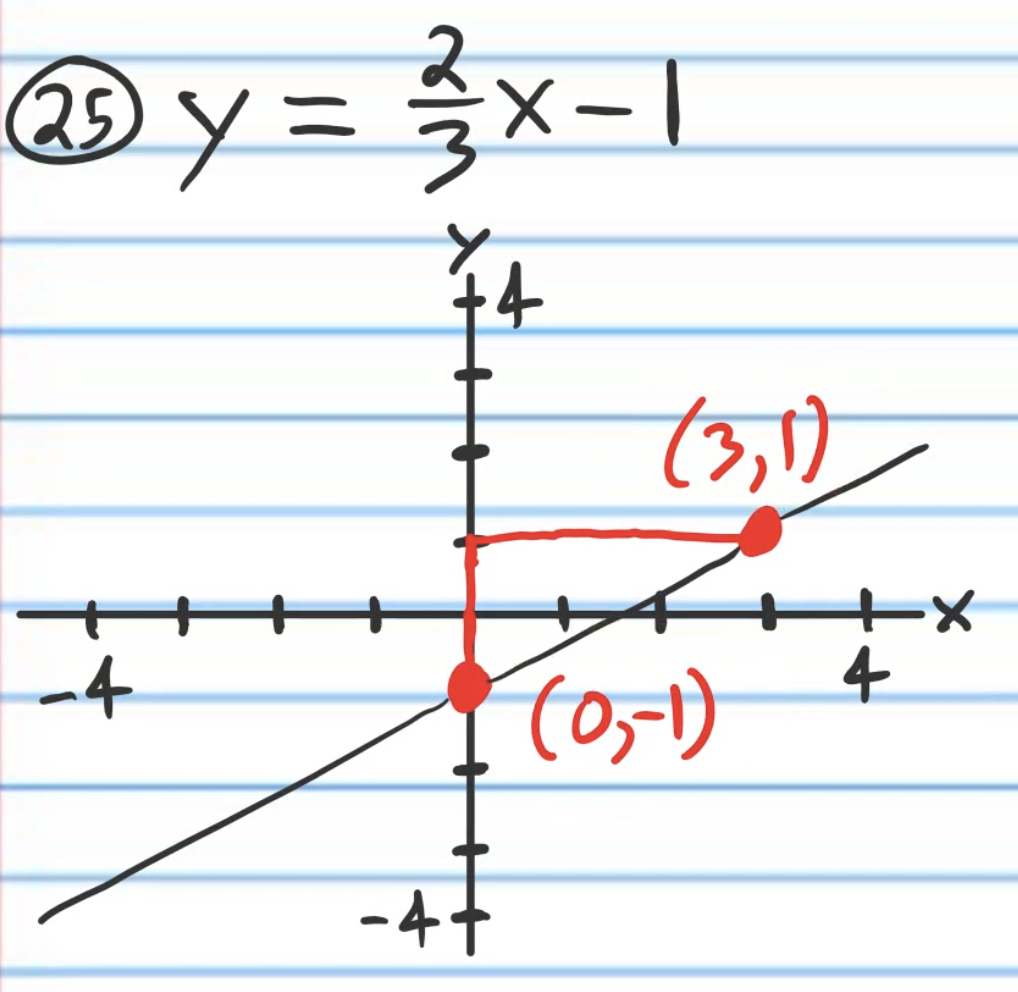
\includegraphics[width=0.5\textwidth]{beg2701.png}
  \caption{The slope is rise/run}
\end{figure}

\newpage

When the slope is a negative number, instead of rising up, we go down and to the right. In the figure below, we go down 4 and then go 5 to the right (một ô đơn vị ứng với 2 units).

\begin{figure}[htb!]
  \centering
  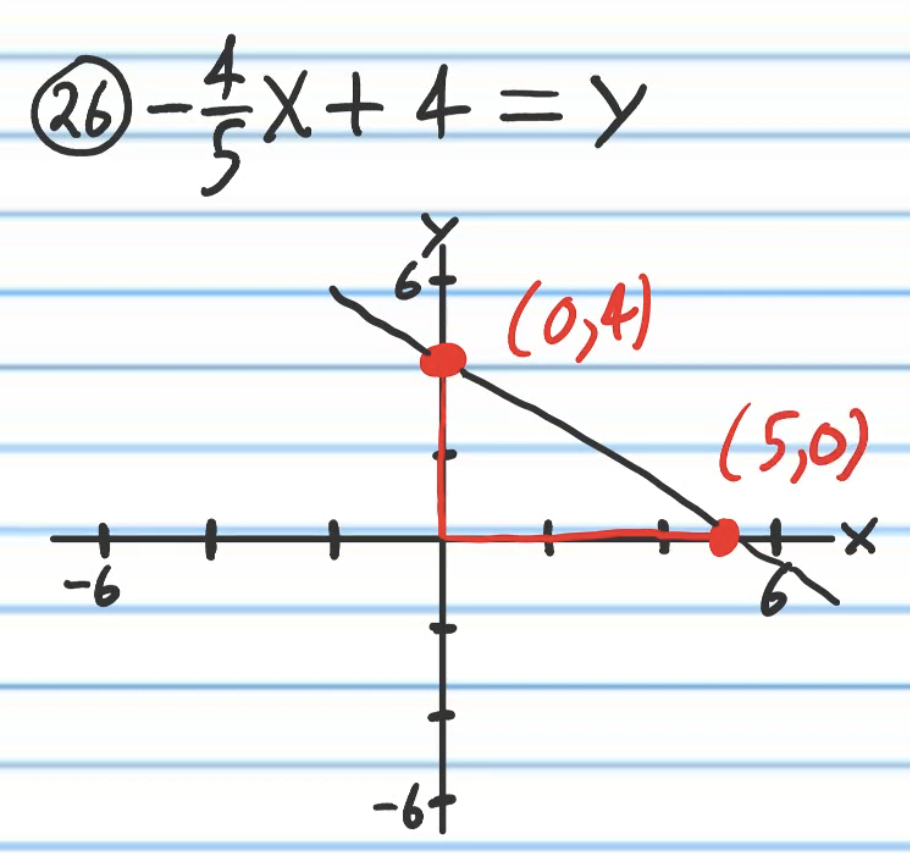
\includegraphics[width=0.5\textwidth]{beg2702.png}
  \caption{When the slope is negative}
\end{figure}

\vspace{0.5cm}

Nếu slope là whole number $2=\frac{2}{1}$. So rise 2 and run 1.

% \vspace{1cm}

Nếu rise \& run chạy ra ngoài hệ trục mình vẽ như trong hình dưới nếu rise 5 and run 3 to the right thì outside the window. Vậy mình sẽ go \textbf{down} 5 and go 3 \textbf{to the left}. Nếu gặp negative slope thì revert bằng cách go up and to the left.

\begin{figure}[htb!]
  \centering
  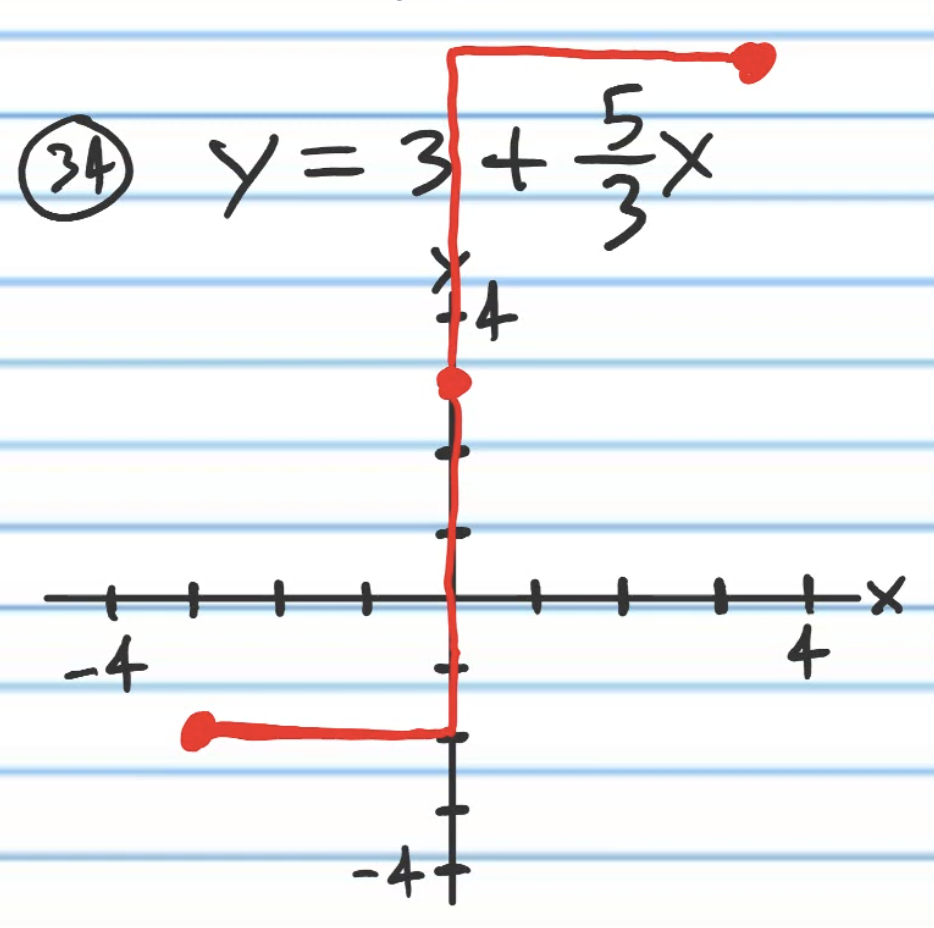
\includegraphics[width=0.5\textwidth]{beg2703.png}
  \caption{Go down and to the left}
\end{figure}

\hl{Method 04}: Using Point-Slope Form. Giống method 03.

\vspace{8mm}

In the problem below, kể cả khi revert the point thì vẫn ra ngoài our drawing window. Vậy thay vì go 3 and 4 whole units of one, we go 3 and 4 half-units of one (tức $\frac{1}{2}$) hoặc 3 and 4 third-units of one ($\frac{1}{3}$. The picture on the right go up three thirds (which is one whole $\frac{3}{3}=1$) and to the left four thirds $\frac{4}{3}$ to get to the x-coordinate $-(2+\frac{4}{3})=-3\frac{1}{3}$ (a mixed number). Chia một unit ra làm 3 phần bằng nhau. Nếu vẫn không đủ nữa thì chia ra fifths.

\begin{figure}[htb!]
  \centering
  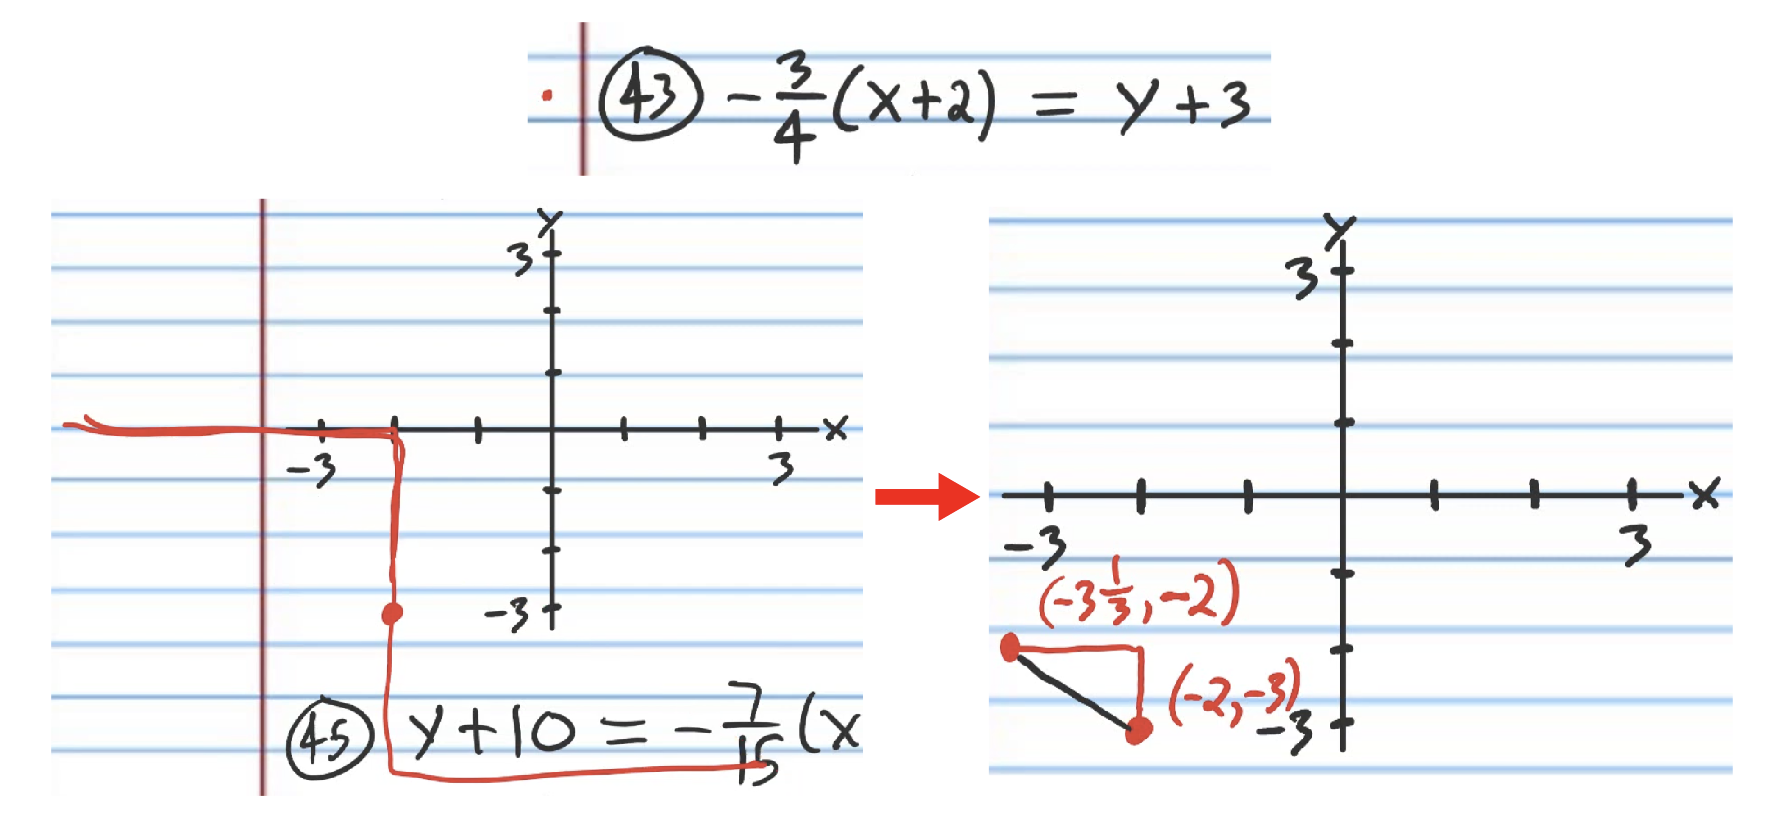
\includegraphics[width=0.9\textwidth]{beg2704.png}
  \caption{Go three thirds}
\end{figure}

\section{Additional Problems on Linear Equations and their Graphs}
% 06 Aug 2025

If two lines are parallel, their slope are equal.

If two lines are perpendicular (vuông góc), the slopes are \textbf{negative reciprocals} ($m_{2}=-(\frac{1}{m_{1}})$). Flip tử mẫu \& đổi dấu.

% Write an equation of the line shown.

\vspace{.4cm}

All Vertical lines like $x=3$ have slope of \textbf{undefined} (mẫu số có denominator chia cho zero).

All Horizontal lines like $y=1$ have slope of \textbf{zero}.

